\pdfoutput=1
\documentclass[a4paper,12pt,titlepage, twoside]{article}
\usepackage[english]{babel}
\usepackage[utf8]{inputenc}
\usepackage{amssymb,amsmath}
\usepackage{algorithm,algpseudocode}
\usepackage[title,titletoc]{appendix}
\usepackage{graphicx}
\usepackage{caption}
\usepackage{subcaption}
\numberwithin{figure}{section}

\begin{document}


% todo: compute Inception accuracy

\section{Introduction}
\subsection{Overview of methodology}
todo...
\subsection{Contribution}
implementing of classical model detections.
using the facenet model for similarities.
Improving the ssd model.


\section{Related work}
state of the art


\section{Image Dewarping}

The fish-eye images are very distorted and standard neural net detectors, which have been pretrained on imagenet, have difficulty correctly recognizing objects. The main idea of this section is 

\subsection{Scene localization}
\label{sec:scene_localization}
Before we start decomposing the image, we need to compensate for another hardware error of the camera. As can be seen in the image \ref{???}, the scene is not exactly in the middle. It is not even circle, but rather an ellipse. Properties of the elipse could be neasured manually, but our system will be deployed on multiple cameras and due to uncertainty in the manufacturing process, each scene has a different location and distortion. Since we need a high precision for further position estimation, an universal algorithm for detecting the sphere has been introduced.

The algorithm is based on optimization. It takes an image and produces parameters of the ellipse. From observation, the ellipse can only be either the horizontal major axis or the vertical major axis ellipse. The used equation is rather unussual, but it allows faster cost function evaluation.

\begin{equation}
\frac{(x-s_x)^2}{a} + \frac{(y-s_y)^2}{1} = r^2
\end{equation}

Now we need to find the parameters $s_x, s_y, a, r$.

The original image $I$ of the size $H, W$ and channels $I_1, I_2, I_3$ is transformed to a mask $M$ of the same size by thresholding the total sum of chanals on 8 bit scale is grather or equal to 1. \cite{lukacs1997real}

\begin{equation*}
M_{x,y} = \begin{cases}
1 & if \quad \sum_{i=1}^{3} I_{i,x,y} \geq 1 \\
0 & otherwise
\end{cases}
\end{equation*}

The mask $M$ represents the scene by the pixels with the value 1 and the background by the pixels with the value 0. 

We create an additional mask $E(s_x, s_y, a, r)$ of the ellipse as 

\begin{equation*}
E_{x,y}(s_x, s_y, a, r) = \begin{cases}
1 & if \frac{(x-s_x)^2}{a} + \frac{(y-s_y)^2}{1} \leq r^2 \\
0 & otherwise
\end{cases}
\end{equation*}

The cost function $C(M, E(s_x, s_y, a, r))$ penalizes the pixels that have been masked as the scene and lie outside the ellipse and the pixels, that have been masked as background and lie inside the ellipse.

\begin{equation}
C(M, s_x, s_y, a, r) = \sum_{x = 0}^{W-1} \sum_{y = 0}^{H-1} E_{x,y}(s_x, s_y, a, r) \cdot (1-M_{x,y}) + (1 - E_{x,y}(s_x, s_y, a, r)) \cdot M_{x,y}
\end{equation}

The algorithm could evaluate all combinations of parameters, but the number of searched parameters can be grately reduced by searching in a coarse to to fine manner. 


\begin{verbatim}
x, y, a, r := initialize_params()
center_step, a_step, r_step := initialize_steps()

while(not imporoving):
    x_list := [x - center_step, x, x + center_step]
    y_list := [y - center_step, y, y + center_step]
    a_list := [a - a_step, a, a + a_step]
    r_list := [r - r_step, r, r + r_step]
    
    x, y, a, r := select_best(x_list, y_list, a_list, r_list)
    
    center_step := center_step / 2
    a_step := a_step / 2
    r_step := r_step / 2
    
return x, y, a, r
\end{verbatim}

This algorithm quickly finds the ellipse with very high precision. Furthermore the most expensive function, $select\_best$ can be highly parallelized.

\section{Fish-eye camera model}
To correctly localize object from the camera, we need to know the transformations between real world coordinates $x^w, y^w, x^w$ and the projection on the captured frame $x^f, y^f$. After applying the algorithm from \ref{sec:scene_localization}, we know, where in the frame the scene is projected. First, we will consider the circle model and at the end we will apply the transformation to ellipse. 

Computing in the cartesian coordinates is not very useful for optics. Instead, the world coordinates are chosen to be spherical and the frame coordinates are chosen to be polar. The world coordinates are in respect to the camera. 
The transformations between the world cartesian coordinates $x^w, y^w, x^w$ and the world spherical coordinates $r^w, \theta^w, \phi^w$ are as follows:

\begin{figure}[h]
\centering
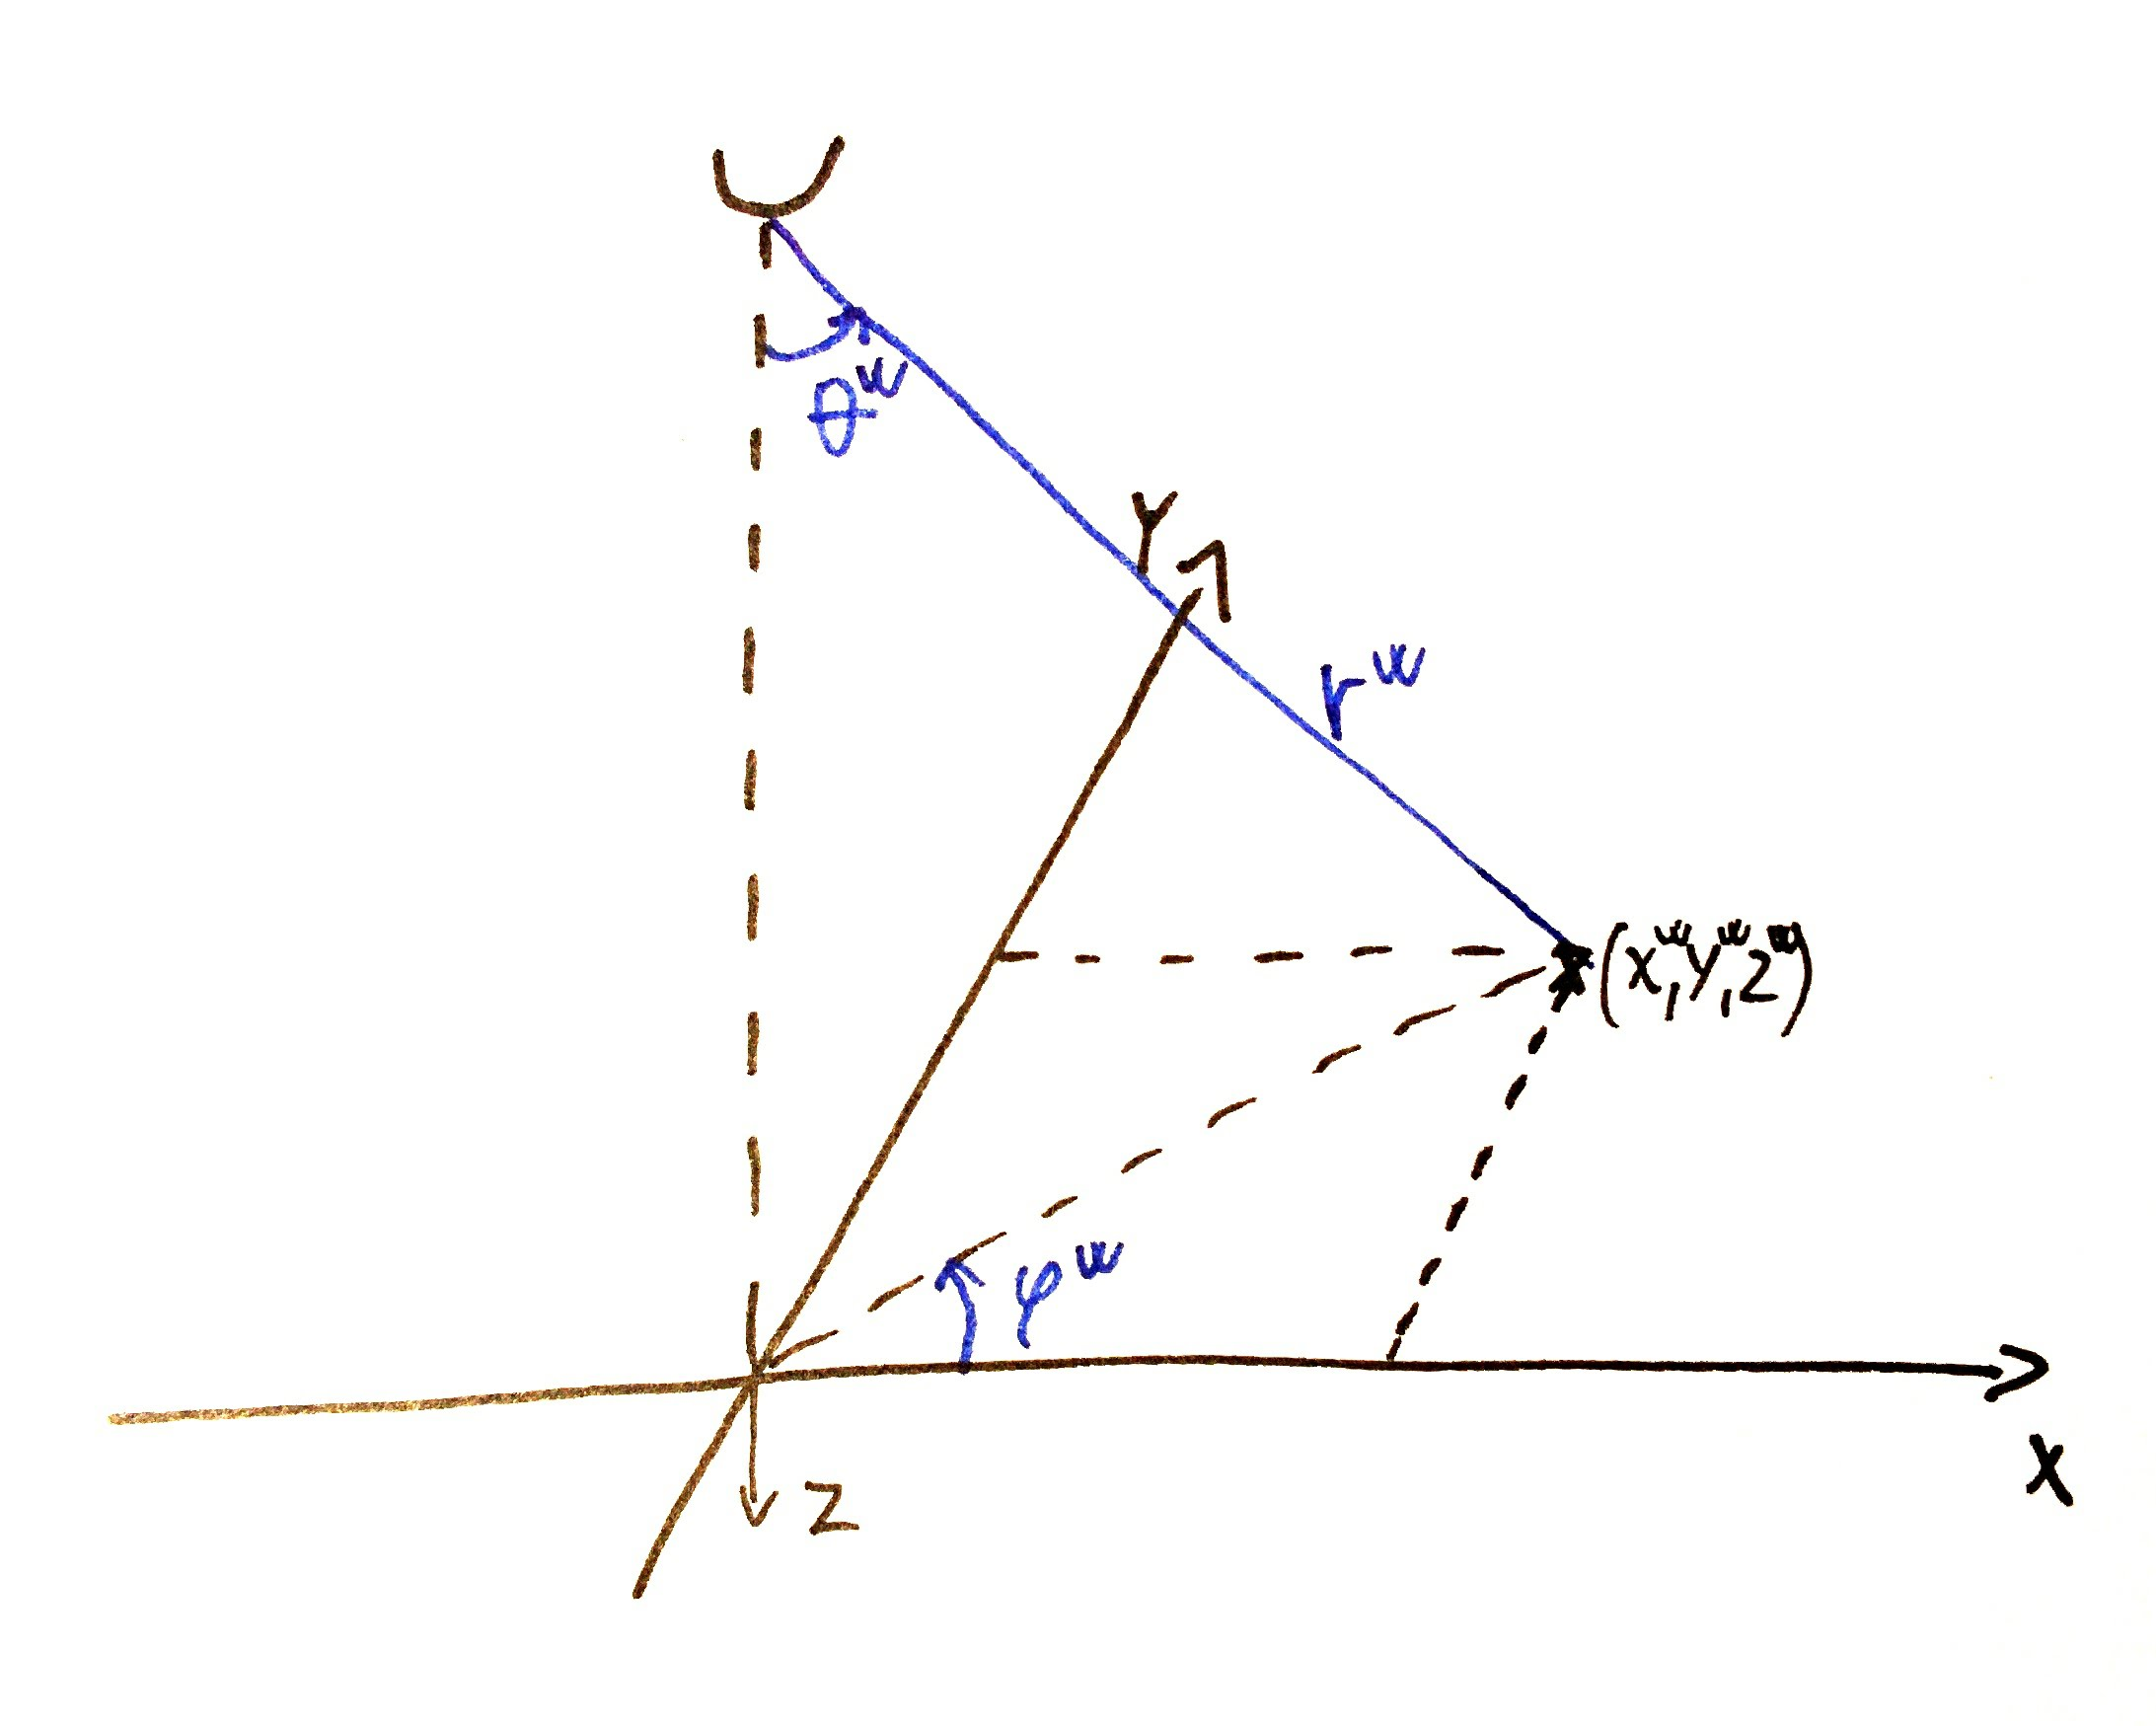
\includegraphics[width=1\linewidth]{fig/sphere.jpg}
\caption{The spherical coordinates of the world}
\label{fig:sphere}
\end{figure}


\begin{equation*}
\begin{aligned}[c]
x^w &= r^w \cdot cos(\theta^w) \cdot sin(\varphi^w) \\
y^w &= r^w \cdot cos(\theta^w) \cdot cos(\varphi^w) \\
z^w &= r^w \cdot sin(\theta^w) \\
\end{aligned}
\qquad,\qquad
\begin{aligned}[c]
r^w &= \sqrt{(x^w)^2 + (y^w)^2 + (z^w)^2} \\
\theta^w &= arcsin\Big(\frac{z^w}{r^w}\Big) \\
\varphi^w &= arctan\Big(\frac{y^w}{x^w}\Big) \\
\end{aligned}
\end{equation*}



The detected scene circle has the radius of $R$ pixels and the center at pixels $s_x, s_y$. The tranformations betwean cartesian frame coordinates $x^f, y^f$ and the polar frame coordinates $r^f, \theta^f$ are:

\begin{equation*}
\begin{aligned}[c]
x^f &= s_x + R \cdot r^f \cdot cos(\varphi^f) \\
y^f &= s_y + R \cdot r^f \cdot sin(\varphi^f) \\
\end{aligned}
\qquad,\qquad
\begin{aligned}[c]
r^f &= \sqrt{(x^f - s_x)^2 + (y^f - s_y)^2} \\
\varphi^f &= arctan\big{(}\frac{y^f - s_y}{x^f - s_x}\big{)}
\end{aligned}
\end{equation*}

Next, we need to find the transformations between the world spheriacal coordinates $r^w, \theta^w, \phi^w$ and the frame polar coordinates $r^f, \theta^f$, but there are some nice properties:

\begin{itemize}
\item The $\varphi$ are the same, i.e. $\varphi^w = \varphi^f$.
\item The transformations do not depend on $r^w$. The projection depends only on the direction, not on the distance from camera.
\end{itemize}

With this knowledge, we need only to find the transformation of $\theta^w$ and $r^f$. We need to find a function $f$, such as 
\begin{equation}
\begin{aligned}
\theta^w &= f(r^f) \\
r^f &= f^{-1}(\theta^w). \\
\end{aligned}
\end{equation}

There are many models for finding $f$. The simplest one is 

\begin{equation}
\theta^w = f(r^f) = \theta^w \cdot FOV,
\end{equation}
where $FOV$ is the field of viw of the camera. Fitting of the model is shown in the fig.\ref{fig:linear_model}


\begin{figure}[h!]
\centering
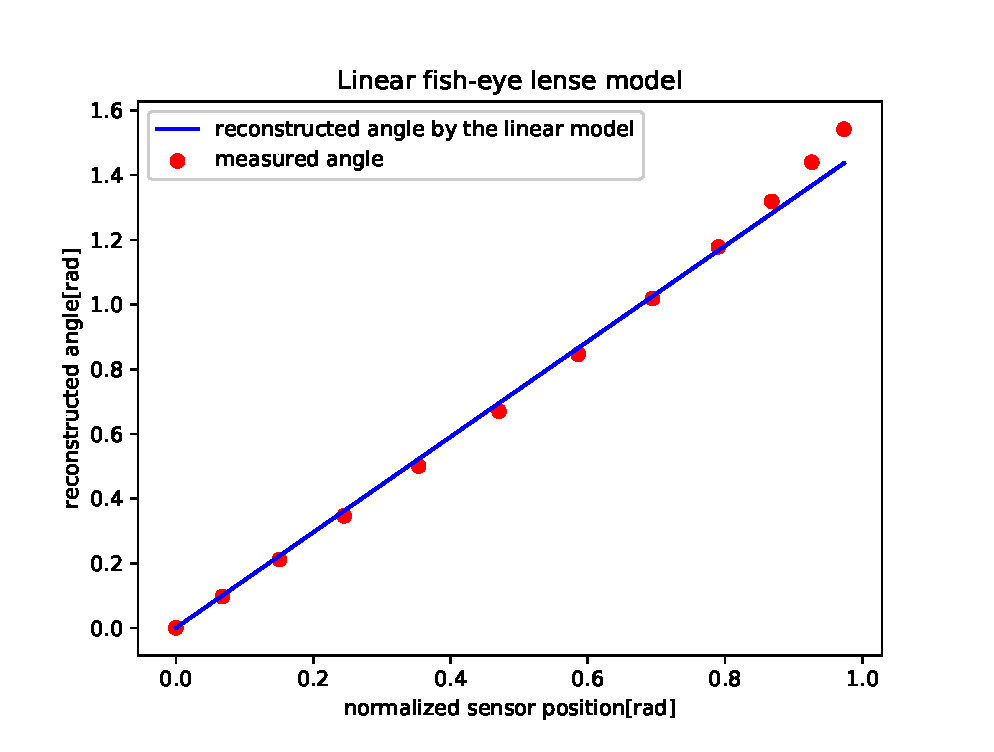
\includegraphics[width=1\linewidth]{fig/linear_model.eps}
\caption{The linear model of the lesnse}
\label{fig:linear_model}
\end{figure}

The linear model estimates the real one quite well and there is no need to search for more complicated model. This model is accurate to about 70$^\circ$ from the radial axis, which is the operational interval of the camera for our purposes.







\section{Detection Evaluation}
For training a neural network, it is important to have some means of evaluating it, so we can compare models. We need to have some algorithm of evaluating the detections on an images against the ground truth. With the detection problem, this is more complicated, than the classification problem.

\subsection{Classification evaluation}

The classification problem is easier than the detection problem. Given the image, predict a class, which is picked from previously known set of classes. The classifier can also return the probability distribution, in which case, the predicted class is the one with the highest probability. There are several metrics for measuring accuracy.

\subsubsection{top 1 accuracy}

The classifier returns the predicted class. If the class matches with the ground truth, the accuracy is 1, therwise it is 0.

\subsection{top 5 accuracy}

Another evaluation is the top 5 accuracy, used for example in imagenet \cite{imagenet} competition. In this evaluation, the detector predicts 5 classes and if the ground truth is among them, it returns 1, otherwise 0. 

\subsection{Mean average precision.}
Mean average precision (mAP) is the most used metrics for object detection problem. The advantage is, that it does not depend on the selected confidence threshold, but only on the IoU threshold. This metrics is not constrained only for object detection problems in vision, but can be used for all detection problems. 

The algorithm for computing mAP runs for all thresholds. Given an arbitrary threshold, the predicted bounding boxes are those, whos confidence exceeds it. If there is a high IoU of a ground truth box and some predicted bounding boxes having the same class, the predicted box with the highest confidence is matched and considered true positive($TP$) and no other box can be matched with the ground truth bounding box. If a predicted bounding box is not matched with any ground truth bounding boxes, it is considered false positive($FP$). If a ground truth bounding box is not matched with any predicted bounding box, it is considered a false negative($FN$).

Precision($P$) corresponds to what portion of ground truth boxes have been matched. With lowering the threshold, it can only increase, sonce more ground truth bounding boxes wiil be matched.
\begin{equation}
P = \frac{TP}{TP + FP}
\end{equation}

Recall($R$) corresponds to what portion of predicted bounding boxes have been matched. 
\begin{equation}
R = \frac{TP}{TP + FN}
\end{equation}

The precision-recall curve in the Fig.\ref{fig:precision-recall} shows the dependency of precision and recall. The higher the precision, the lower the recall. The area below the curve is called averge precision($AP$) and the mean over all classes is called mean average precision($mAP$).

\begin{equation}
mAP = \frac{1}{|C|} \sum_{c \in C} AP_c
\end{equation}

where $C$ is the set of classes.

\begin{figure}[h]
\centering
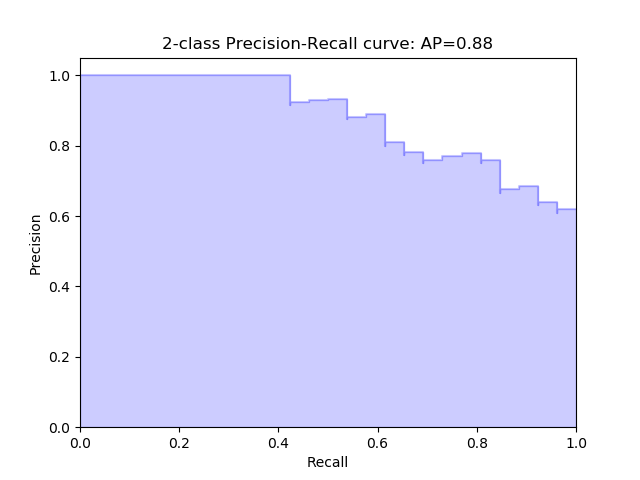
\includegraphics[width=1\linewidth]{fig/precision-recall.png}
\caption{Precision-recall curve}
\label{fig:precision-recall}
\end{figure}




\section{Background Subtraction}
We can use the fact, that the camera is static. This brings more information and the vehicles can be detected with the background subtraction algorithm. The main idea is creating a model of the scene without vehicles and then subtracting the current frame and by thresholding determine, where the vehicles are. This simple approach would not work very well and some improvements need to be made. 

The algorithm has been implemented in opencv \cite{opencv}. The background is usually created by the mean over several images \cite{bs1, bs2}. It is also updated with each new frame as a weighted sum. The background looks like a photo with a long exposition and the lane, where vehicles drive has a colored lines. This is very bad for thresholding, when the whole lane or nothing is detected. A new approach has been introduced, as taking the median instead of the mean. This turns out to work much better, but still has it's limits. If the traffic is very high and vehicles occupy in average more than half of the ground, the background model will fail completely. Some more complicated models based on unsupervised learning could be used, but they would be computationally too complex and would not work for realtime video.



\begin{figure}
    \begin{subfigure}[Sample1]{0.5\linewidth}
        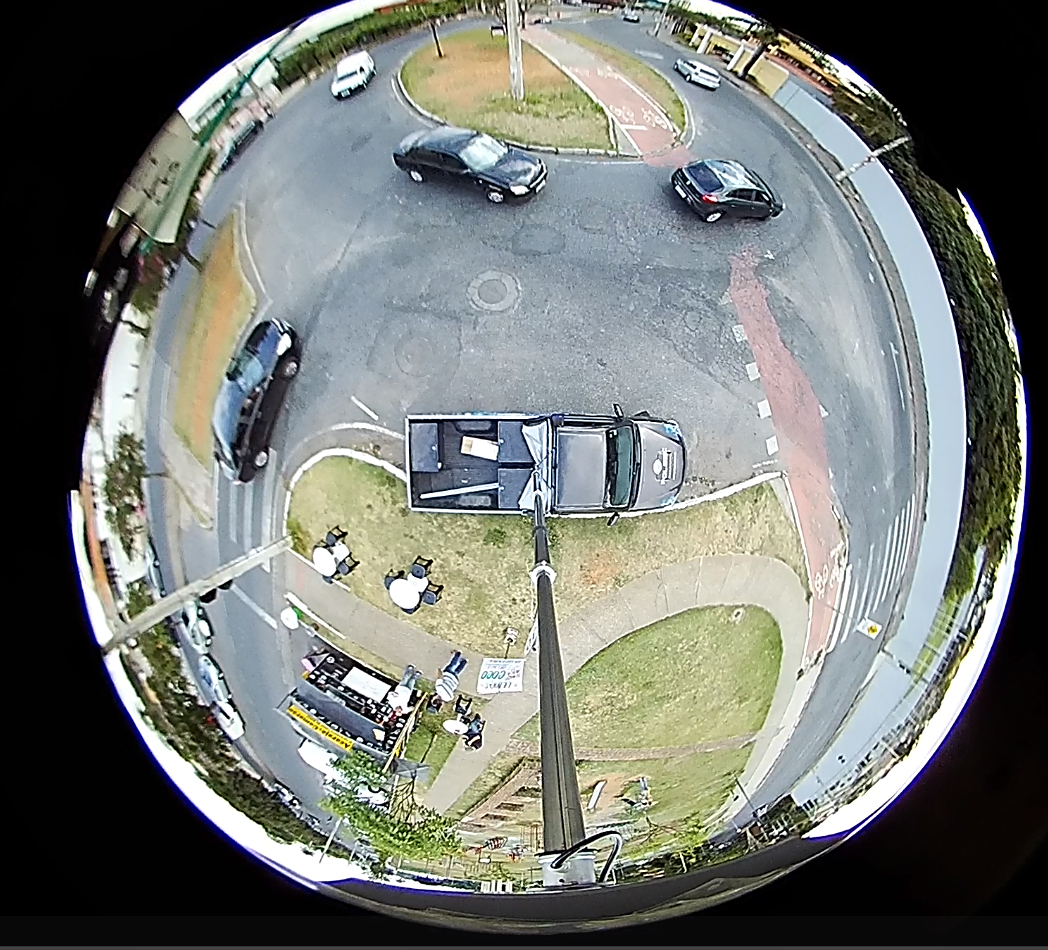
\includegraphics[height=65mm]{fig/frame.png}
        \label{fig:a}
        \caption{A video frame}
    \end{subfigure}
    \qquad
    \begin{subfigure}[Sample1]{0.5\linewidth}    
        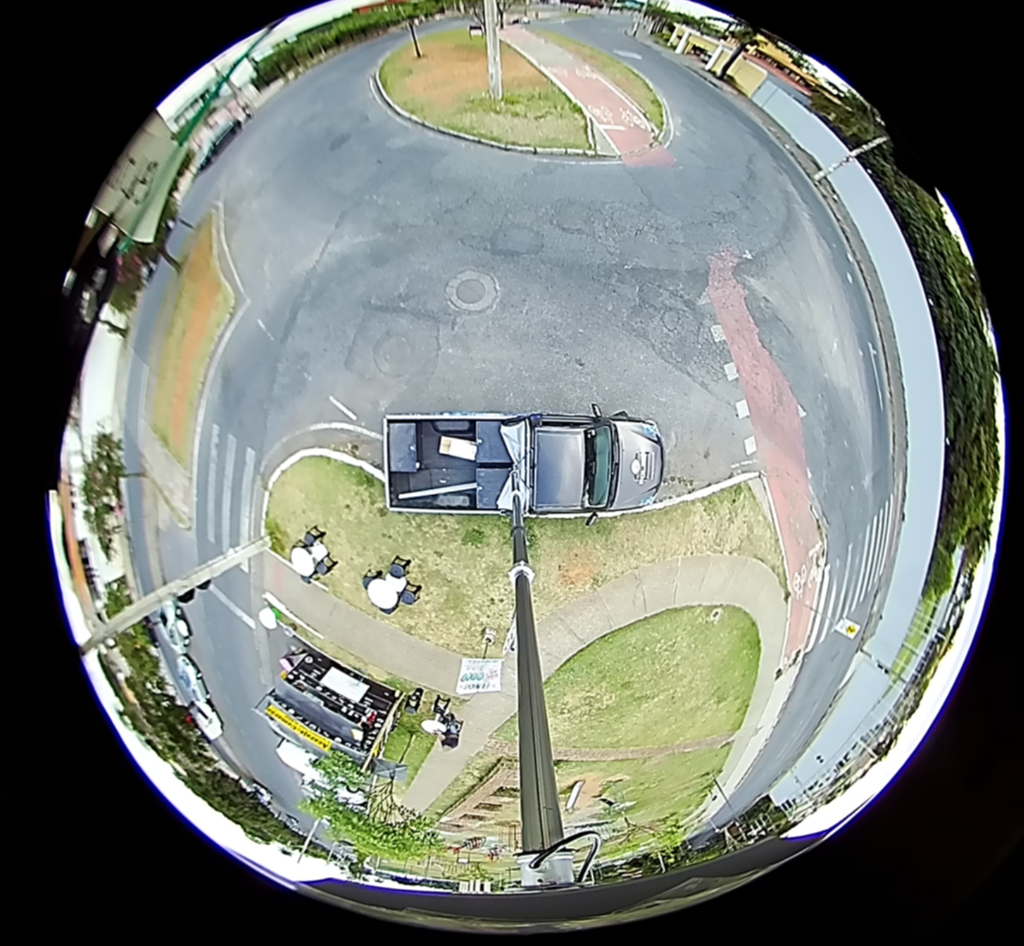
\includegraphics[height=65mm]{fig/background.png}
        \label{fig:b}    
        \caption{The background created using median}
    \end{subfigure} 
    \caption{my caption}
\end{figure}



The difference between background model and the current frame is very noisy and some filtration has to be made. Before subtraction, the background and the frame has been filtrated with a gaussian filter with the size 3x3 for smoothing. Then smoothed again with the filter 11x11. This image is then thresholded and a mask is obtained. Each blob is presented with a contour and they are thresholded once more by the area. The resulted blobs become detections and a bounding box is created.

The background must be continuously adapting to the scene, but the rate of adapting is crucial. If the background is changing too slowly, it will not work very well with changes of lightning from coming clouds, etc. If the background adapts too fast, it will start to contain cars, that stop at the cross section and when the cars leave, this will become a new false detection. From experiments, there is no optimal adapting rate and it depends on the scene, weather and even then these problems will not completely disappear. One small advantage is filtering detections while adapting background.

Background subtraction has many more downsides. Moving trees and shadows create false positives and overlapping objects are represented as one. 

For these problems, background subtraction alone can't be used as a good detector. However, if the conditions are perfect, that means very low traffic for non overlapping vehicles and successful background learning, non changing weather and few trees and their many shadows, the background subtraction works very well. On these scenes, this can be very useful for collecting high quality training data for neural networks. 

\section{Optical Flow}
A custom set of algorithms has been implemented in opencv\cite{opencv} for improving the background subtraction problems.  Optical flow \cite{optical-flow} is not used over the whole image, since that would be too expensive. Instead, each detection is extended for a one optical flow point. In the next frame, this point will move with the object. This extends the detector for object tracking and partially solves the problem of two overlapping vehicles. If two vehicles drive close to each other, background subtraction would start to treat them as one object. This improved model will detect this situation and keep the bounding boxes on the different vehicles. 

There is a set of rules, but these are the main ones:
\begin{itemize}
	\item If an optical flow point is outside the background subtraction mask, it becomes a 'zombie'.
	\item If a background subtraction detection is without an optical flow point and there is no 'zombie' in the detection, optical flow point is created in the middle of the bounding box. 
	\item If a zombie is not recovered in 10 frames, it disappears. 
	\item If there are more optical flow points in one background subtraction detection, the bounding boxes continue movement with a low pass filter.
	\item The optical flow points are forced to the middle of the bounding box. This solves the problem of the detection being put on the front of the car while coming and due to noise later being outside the bounding box, when the vehicle is viewed from a side.
\end{itemize}

These improvements work surprisingly well and solve the tracking problem to some extent. If vehicles overlap completely, this approach will fail, but so will most of the other ones. 









\bibliographystyle{plain}
\bibliography{ref}{}
\cleardoublepage
\clearpage

\end{document}